\documentclass[slidestop,compress,mathserif]{beamer}

\usepackage{kotex}
\usepackage{graphicx}
\usepackage{authblk}
\usepackage{mdframed}
\usepackage{amsmath}
\usepackage{amsfonts}
\usepackage{amsthm}
\usepackage{mathrsfs}
\usepackage{setspace}
\usepackage{proof}
\usepackage{hyperref}

\title{람다-프롤로그로 나만의 타입체커 만들기}
\author{임기정}

\hypersetup{ colorlinks=true, linkcolor=blue, filecolor=magenta, urlcolor=cyan, }

\newenvironment{nemochang}
{
    \begin{center}
    \begin{tabular}{|p{0.95\textwidth}|}
    \hline
    \vspace{0.1em}
}
{
    \hline
    \end{tabular}
    \end{center}
}

\begin{document}
    \begin{frame}
        \titlepage
    \end{frame}

    \begin{frame}
        \frametitle{서론}
        \begin{itemize}
            \item 타입체커를 쉽게 만들고자 하시는 분들을 위해 발표합니다!
            \pause
            \item System-F:
            \begin{enumerate}
                \item 단순 타입 람다-계산법에 타입에 대한 보편 양화사를 추가한 시스템입니다.
                \item 하스켈과 ML 같은 함수형 언어의 이론적 기반입니다.
            \end{enumerate}
            \pause
            \item 논리형 프로그래밍:
            \begin{enumerate}
                \item \textit{규칙}이라 불리는 논리식들을 작성하는 프로그래밍 패러다임입니다.
                \item 그리하여 인터프리터가 주어진 규칙들로부터 질의받은 논리식을 증명할 수 있는지를 응답합니다.
            \end{enumerate}
            \pause
            \item 람다-프롤로그:
            \begin{enumerate}
                \item 함수 타입의 논리 변수를 허용하는 논리형 프로그래밍 언어입니다.
                \item 규칙이 될 수 있는 논리식의 꼴이 프롤로그에서는 Horn clause인 반면, (새로운) 람다-프롤로그에서는 higher-order hereditary Harrop입니다.
            \end{enumerate}
        \end{itemize}
    \end{frame}

    \begin{frame}
        \frametitle{$L_\lambda$에 대한 간단한 소개}
        \begin{itemize}
            \item 1991년에 Dale Miller는 Teyjus V2의 이론적 기반이 될 논리형 언어 $L_\lambda$를 발표했습니다.
            \item 함수 타입의 논리 변수의 나타남에 특정한 제약을 가했기 때문에, 이 언어의 구현체는 고차 단일화 문제들 중 higher-order pattern unification이라고 불리는 특수한 문제들만 풀면 됩니다.
            \item 2009년에 Xiaochu Qi는 (새로운) 람다-프롤로그의 구현체 Teyjus V2를 개발하는 데 성공했는데, 기존의 Teyjus가 단일화 문제를 Huet's Algorithm으로 푸는 반면 V2는 Nadathur와 Linnell이 제안한 알고리즘으로 풉니다.
            \item \href{https://github.com/teyjus/teyjus/releases}{Teyjus V2의 깃허브 페이지에서} 컴파일러 `tjcc', 링커 `tjlink' 그리고 시뮬레이터 `tjsim'를 다운받을 수 있습니다.
        \end{itemize}
    \end{frame}

    \begin{frame}
        \frametitle{그 특정 제약이란 무엇인가? - 1}
        \begin{itemize}
            \item $L_\lambda$의 타입 시스템은 단순 타입 람다-계산법입니다.
            \item $o$: 기저 타입으로서 명제들의 타입을 의미합니다.
            \item 술어 타입: $\tau_1 \to \cdots \to \tau_n \to o$ 꼴의 타입인데, 여기서 $n \geq 0$이고 $\tau_1$, ..., $\tau_n$ 중 $o$를 포함한 타입이 없어야 합니다.
            \item 술어: 술어 타입의 상수를 의미합니다.
            \item 시그니처: 각 상수를 그것의 타입으로 보내는 맵입니다.
            \item 상수 $c$가 시그니처 $\Sigma$의 키가 아니라면, $\Sigma \cup \left\{ \left( c , \tau \right) \right\} $를 $\Sigma + c : \tau$라고 표기합니다.
        \end{itemize}
    \end{frame}

    \begin{frame}
        \frametitle{그 특정 제약이란 무엇인가? - 2}
        \begin{itemize}
            \item $A$를 $p \, t_1 \, \cdots \, t_n$ 꼴의 $\Sigma$-항을 나타내도록 하되, 여기서 $p$는 술어여야 하고, $t_1$, ..., $t_n$ 모두 자유변수를 가지지 않아야 합니다.
            \item Dale Miller는 $\Sigma$-논리식을 다음과 같이 귀납적으로 정의했습니다:
            \begin{enumerate}
                \item $A$는 $\Sigma$-논리식이다.
                \item $B$와 $C$가 $\Sigma$-논리식이면 $B \land C$와 $B \supset C$도 $\Sigma$-논리식이다.
                \item $B \left[ x := c \right]$가 $\left( \Sigma + c : \tau \right)$-논리식이고 $\tau$가 $o$를 포함하지 않으면, $\forall_{\tau} x . B$도 $\Sigma$-논리식이다.
            \end{enumerate}
            \item 모든 $\Sigma$-논리식들은 닫혀있음에 유의하십시오. 즉, $\Sigma$-논리식에서 변수의 자유로운 나타남은 없습니다.
            \item 그리고서 그는 다음과 같이 질의가 될 수 있는 $\Sigma$-논리식을 $G$로, 규칙이 될 수 있는 $\Sigma$-논리식을 $D$로 두었습니다.
            \begin{enumerate}
                \item $G \, ::= \, A \, | \, G \land G \, | \, D \supset G \, | \, \forall_{\tau} x . G$.
                \item $D \, ::= \, A \, | \, D \land D \, | \, G \supset D \, | \, \forall_{\tau} x . D$.
            \end{enumerate}
        \end{itemize}
    \end{frame}

    \begin{frame}
        \frametitle{그 특정 제약이란 무엇인가? - 3}
        \begin{itemize}
            \item $\forall_{\tau} x . G$에서 $\forall_{\tau}$에 묶인 변수 $x$를 \textit{본질적으로 보편 양화}되었다고 합니다.
            \item $\forall_{\tau} x . D$에서 $\forall_{\tau}$에 묶인 변수 $x$를 \textit{본질적으로 존재 양화}되었다고 합니다.
            \item ((논리식 레벨이 아닌) 항-레벨에서) $\lambda$에 묶인 변수를 \textit{본질적으로 보편 양화}되었다고 합니다.
            \item 그 특정 제약은 모든 $\Sigma$-논리식 $B$에 대하여 $x \, y_1 \, \cdots \, y_n$가 $B$의 부분항이고 (단, $n \geq 0$) $x$이 본질적으로 존재 양화되었다면, $y_1$, ..., $y_n$은 다음 조건들을 만족시키는 변수들의 리스트여야 합니다:
            \begin{enumerate}
                \item $y_1$, ..., $y_n$ 모두 본질적으로 보편 양화될 것.
                \item $y_1$, ..., $y_n$ 모두 $x$보다 더 안쪽의 스코프에 있을 것.
                \item $y_1$, ..., $y_n$은 서로 다른 변수들일 것.
            \end{enumerate}
            \item 그러한 부분항들 중 $n \geq 1$인 것들을 \textit{고차 패턴}이라 불립니다.
        \end{itemize}
    \end{frame}

    \begin{frame}
        \frametitle{고차 패턴이 아닌 것들}
        \begin{itemize}
            \item 예 1: $x$와 $y$가 본질적으로 존재 양화되었다면, $x \, y$는 고차 패턴이 아닙니다. (규칙 1 위반)
            \item 예 2: $x$가 본질적으로 존재 양화되고 $c$가 본질적으로 보편 양화되어도, $x$가 $c$를 볼 수 있다면 $x \, c$는 고차 패턴이 아닙니다. (규칙 2 위반)
            \item 예 3: $x$가 본질적으로 존재 양화되고 $c$가 본질적으로 보편 양화되어도, $x \, c \, c$는 고차 패턴이 아닙니다. (규칙 3 위반)
            \item 예 4: $x$가 본질적으로 존재 양화되고 $c$와 $d$가 본질적으로 보편 양화되어도, $x \left( c \, d \right)$는 고차 패턴이 아닙니다. ($ c \, d$가 변수가 아니라 합성항이기 때문)
            \item 이렇게 고차 패턴만 다루었을 때 장점은 다음과 같습니다:
            \begin{enumerate}
                \item 단일화 알고리즘이 결정가능하다. 즉, 무한 루프에 절대 빠지지 않고, 유한 절차 안에 (성공했는지 실패했는지) 결과가 나온다.
                \item 단일화 가능하다면, most general unifier를 얻을 수 있다.
            \end{enumerate}
        \end{itemize}
    \end{frame}

    \begin{frame}
        \frametitle{구문론과 의미론 - 1}
        \begin{itemize}
            \item 이제 본격적으로 (새로운) 람다-프롤로그의 구문론과 작동의미론을 공부해봅시다.
            \item 먼저, (새로운) 람다-프롤로그의 구문은 higher-order hereditary Harrop 논리식으로 볼 수 있는데, 앞서 공부한 $L_\lambda$의 구문론을 확장한 것입니다:
            \begin{enumerate}
                \item $G \, ::= \, \top \, | \, A \, | \, G \land G \, | \, G \lor G \, | \, \exists x . G \, | \, \forall x . G \, | \, D \supset G$.
                \item $D \, ::= \, A_r \, | \, G \supset A_r \, | \, D \land D \, | \, \forall x . D$.
                \item $A \, ::= \, P \, | \, A \, t$, 여기서 항 $t$에 나타날 수 있는 논리 연산자는 $\land$, $\lor$, $\exists$와 $\forall$뿐이고, 항 $P$는 변수 또는 상수여야 함.
                \item $A_r \, ::= \, P \, | \, A \, t$, 여기서 항 $t$에 나타날 수 있는 논리 연산자는 $\land$, $\lor$, $\exists$와 $\forall$뿐이고, 항 $P$는 상수여야 함.
            \end{enumerate}
            \item 물론, 여전히 $G$는 질의받은 논리식을 나타내고, $D$는 규칙으로서의 논리식을 나타냅니다.
            \item 또한, $A$와 $A_r$의 타입 역시 $o$여야 함은 당연합니다.
        \end{itemize}
    \end{frame}

    \begin{frame}
        \frametitle{중략}
        to do ...
    \end{frame}

    \begin{frame}
        \frametitle{타입의 표현}
        \begin{itemize}
            \item 우선 
        \end{itemize}
    \end{frame}

    \begin{frame}
        \frametitle{최종 인터페이스}
        \begin{figure}[h]
            \begin{center}
                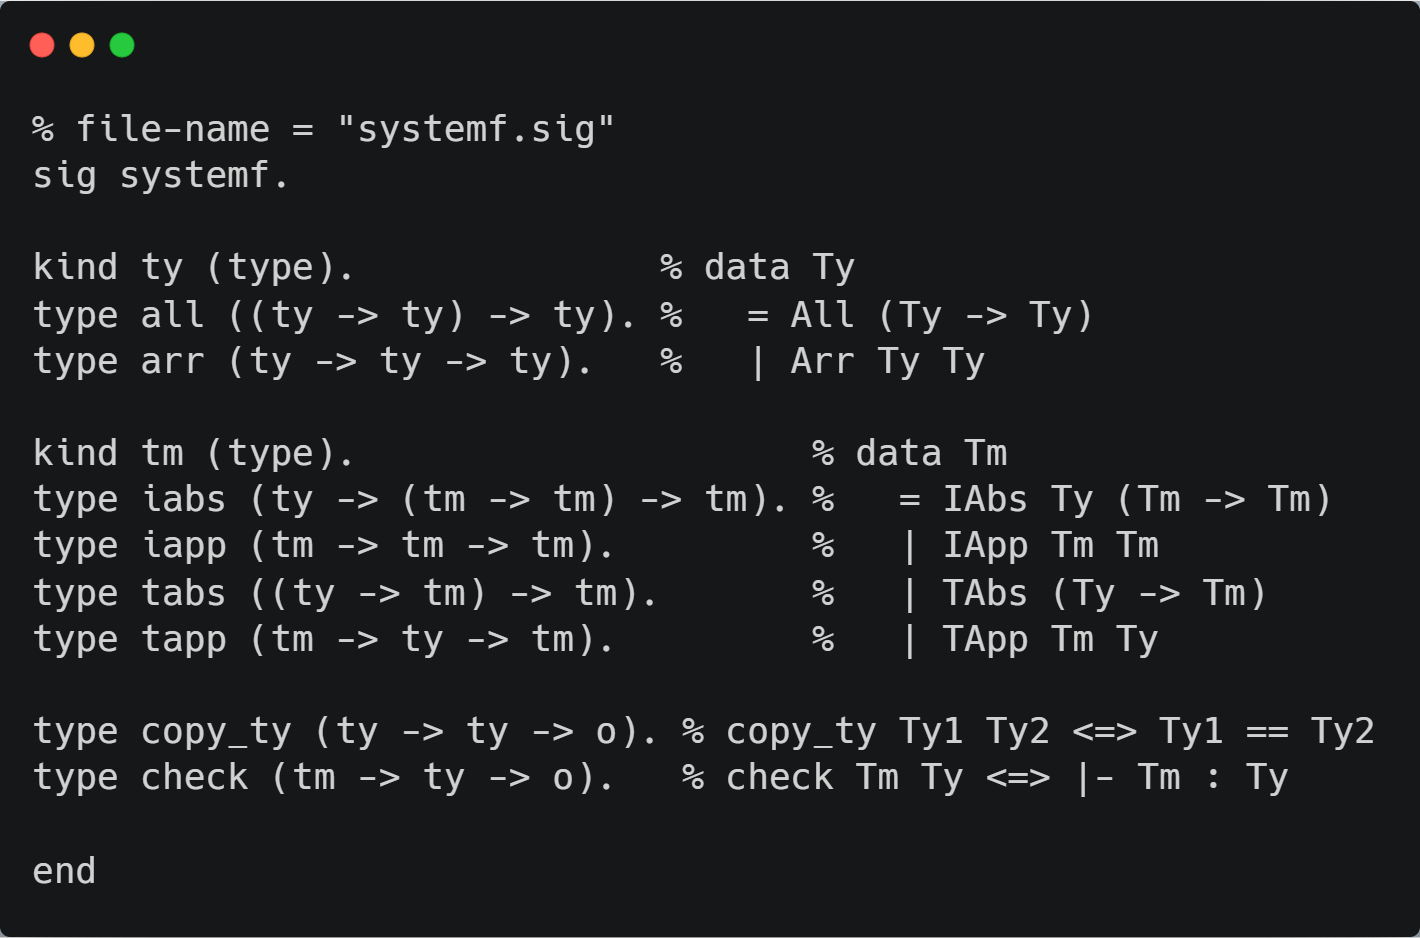
\includegraphics[width=0.7\linewidth]{sig.png}
            \end{center}
        \end{figure}
        \begin{itemize}
            \item 논의한 바를 종합하면, 위와 같습니다.
            \item 파일명은 \texttt{systemf.sig}로 해주세요!
        \end{itemize}
    \end{frame}

    \begin{frame}
        \frametitle{중략}
        to do ...
    \end{frame}

    \begin{frame}
        \frametitle{최종 구현}
        \begin{figure}[h]
            \begin{center}
                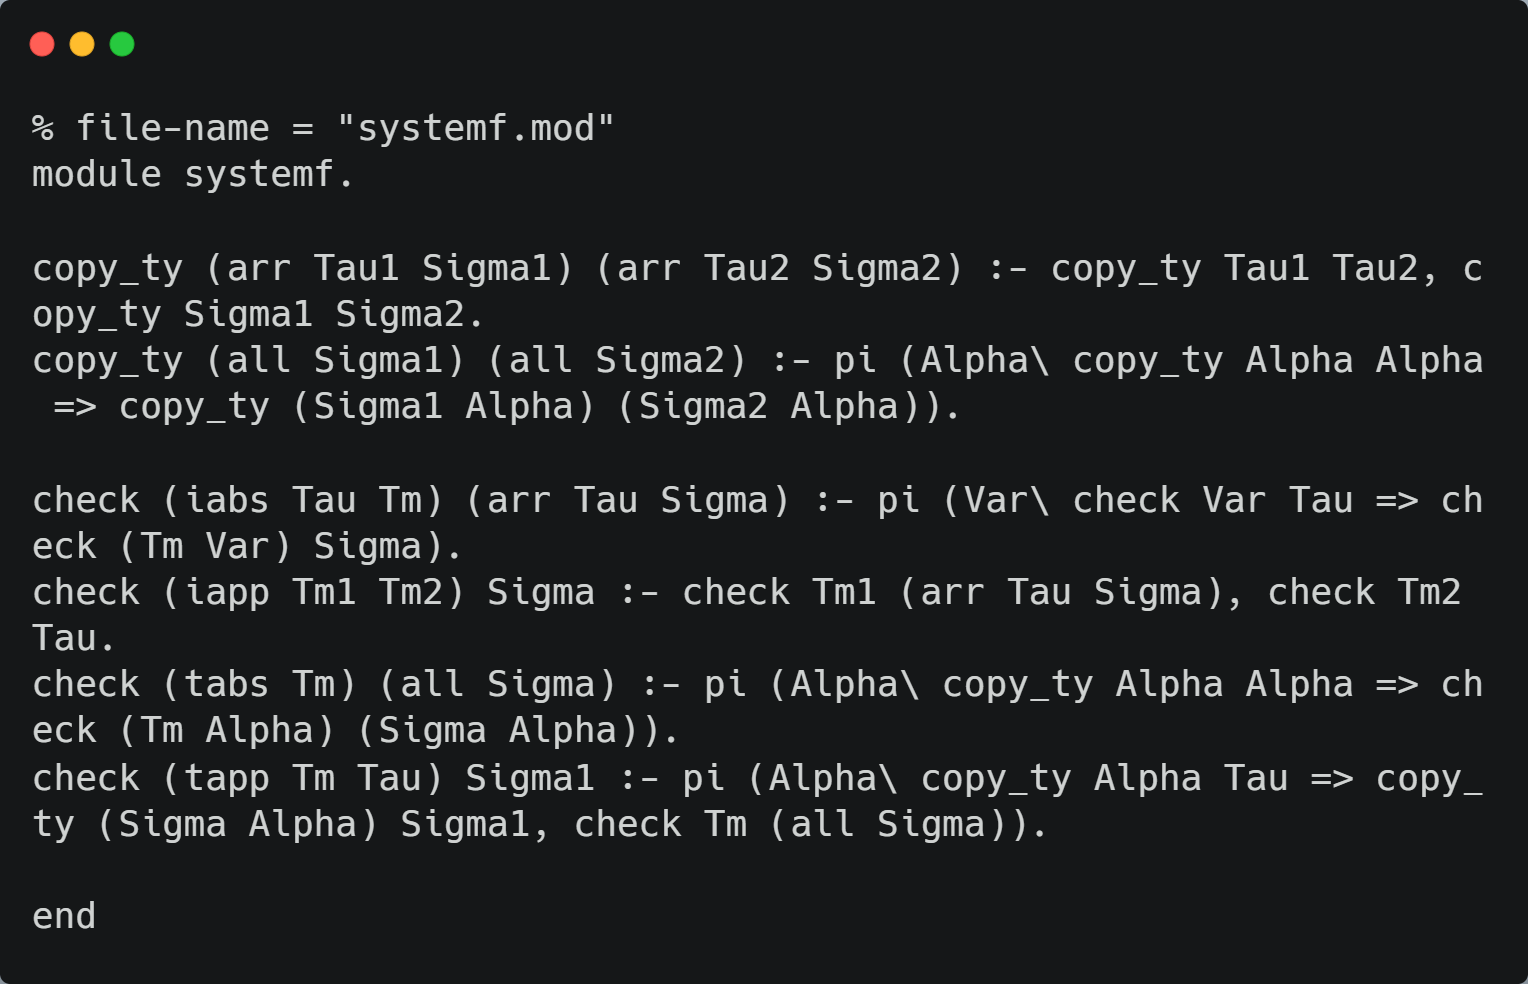
\includegraphics[width=1.0\linewidth]{mod.png}
            \end{center}
        \end{figure}
        \begin{itemize}
            \item 우와! 구현이 12줄만에 타입체커를 짤 수도 있군요.
            \item 파일명은 \texttt{systemf.mod}로 해주세요!
        \end{itemize}
    \end{frame}

    \begin{frame}
        \frametitle{이제 실행해봅시다.}
        \begin{figure}[h]
            \begin{center}
                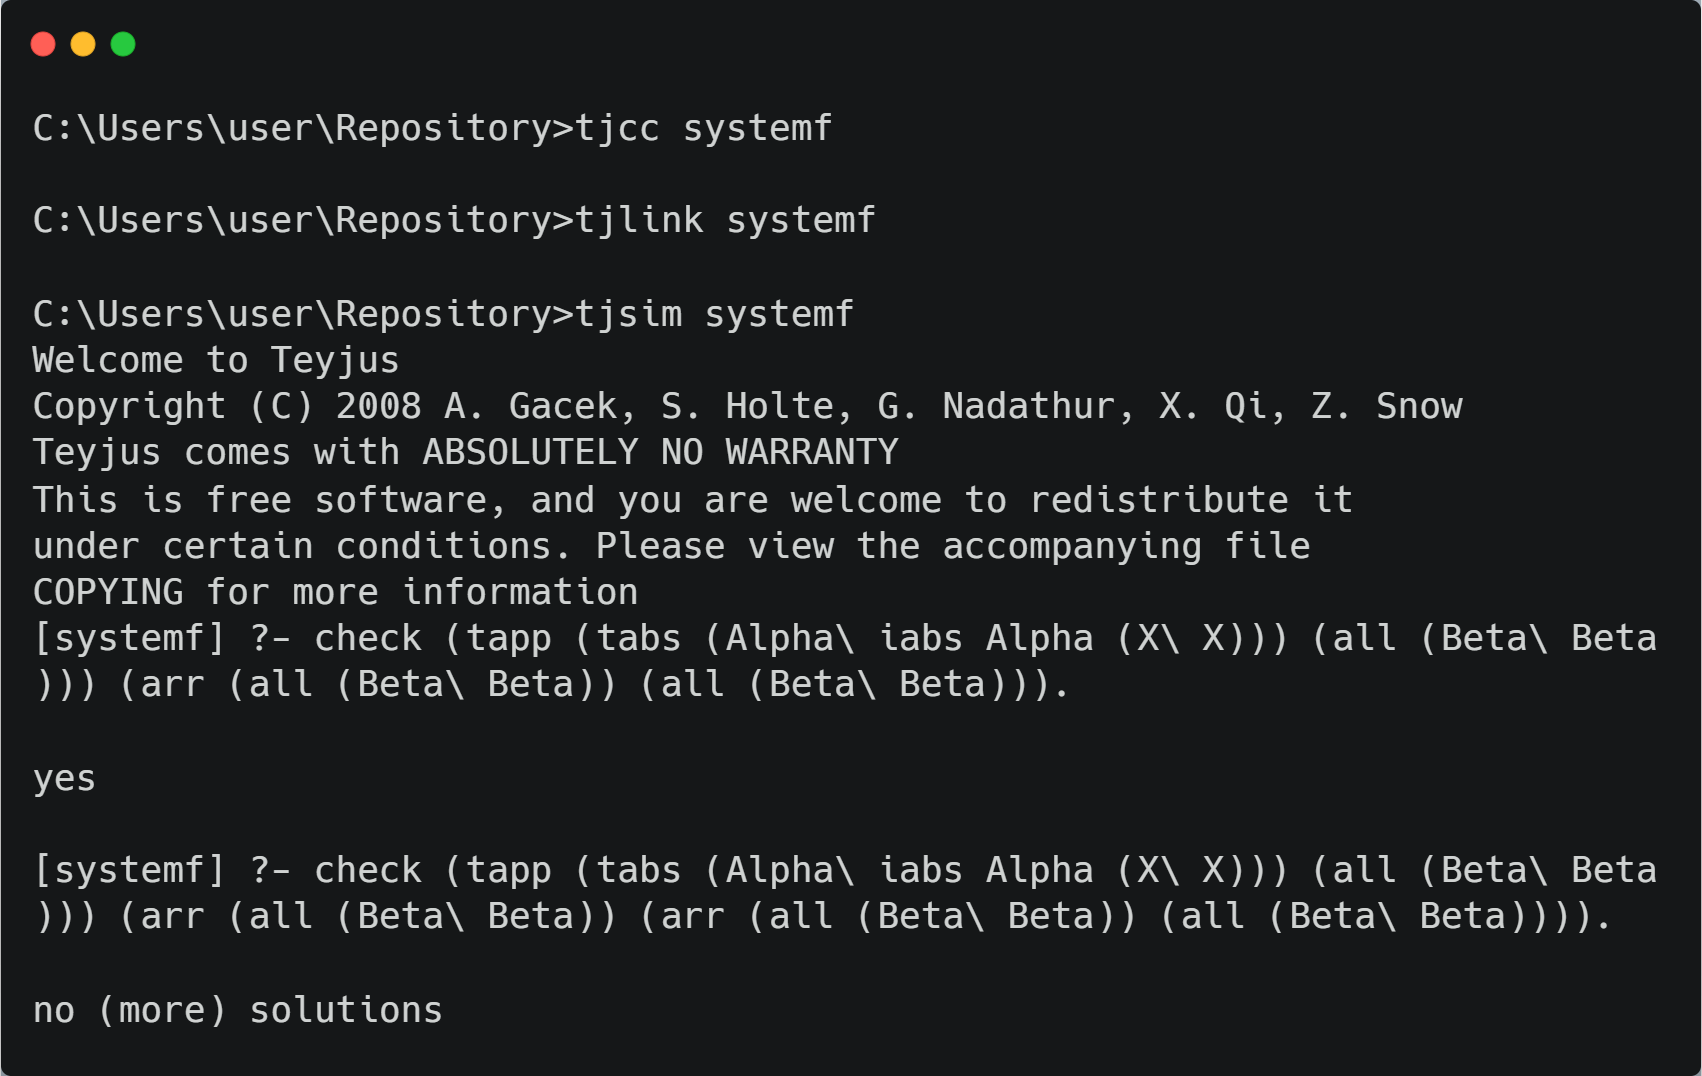
\includegraphics[width=0.9\linewidth]{fin.png}
            \end{center}
        \end{figure}
        \begin{itemize}
            \item 먼저 ``tjcc systemf''라고 치시고, ``tjlink systemf''라고 치신 다음, ``tjsim systemf''라고 치시면, 인터프리터가 실행됩니다.
        \end{itemize}
    \end{frame}

    \begin{frame}
        \frametitle{이제 실행해봅시다.}
        \begin{figure}[h]
            \begin{center}
                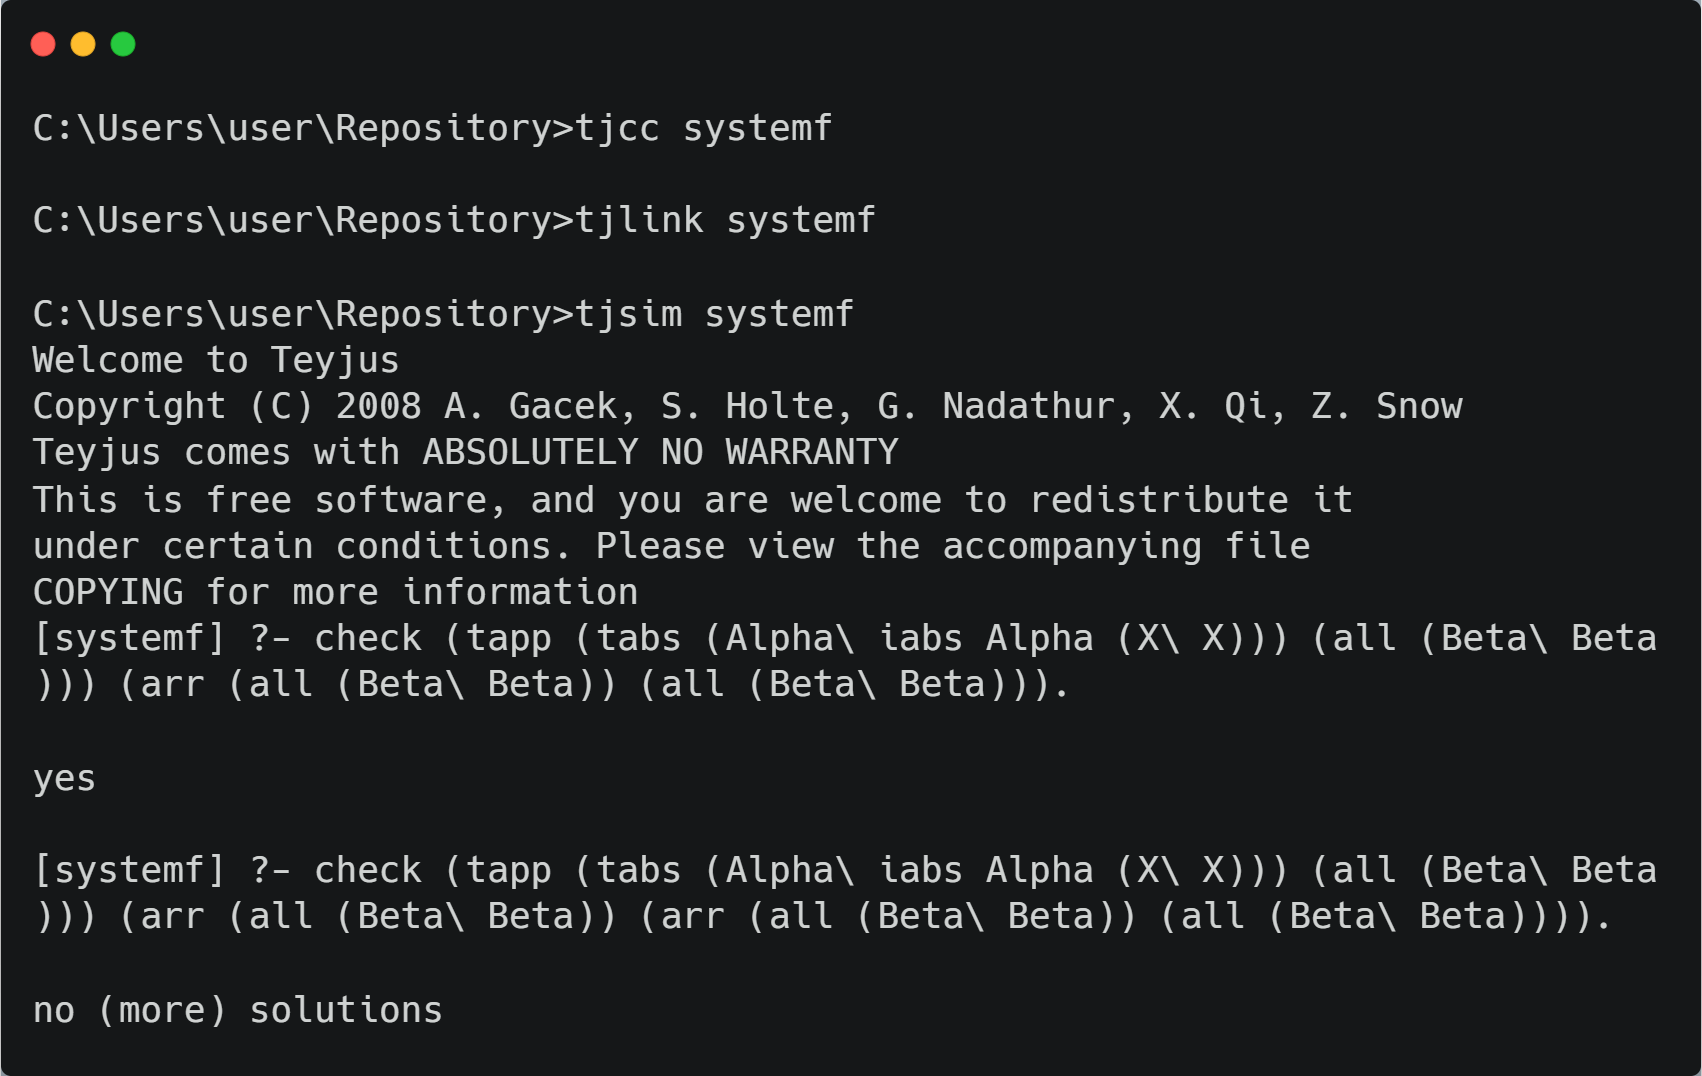
\includegraphics[width=0.9\linewidth]{fin.png}
            \end{center}
        \end{figure}
        \begin{itemize}
            \item 첫 번째로 $\vdash \left( \Lambda \alpha . \lambda x^{\alpha} . x \right) \left( \forall \beta . \beta \right) : \left( \forall \beta . \beta \right) \to \left( \forall \beta . \beta \right)$인지 질의해보겠습니다.
            \item Teyjus V2는 ``yes''라고 응답하는군요.
        \end{itemize}
    \end{frame}

    \begin{frame}
        \frametitle{이제 실행해봅시다.}
        \begin{figure}[h]
            \begin{center}
                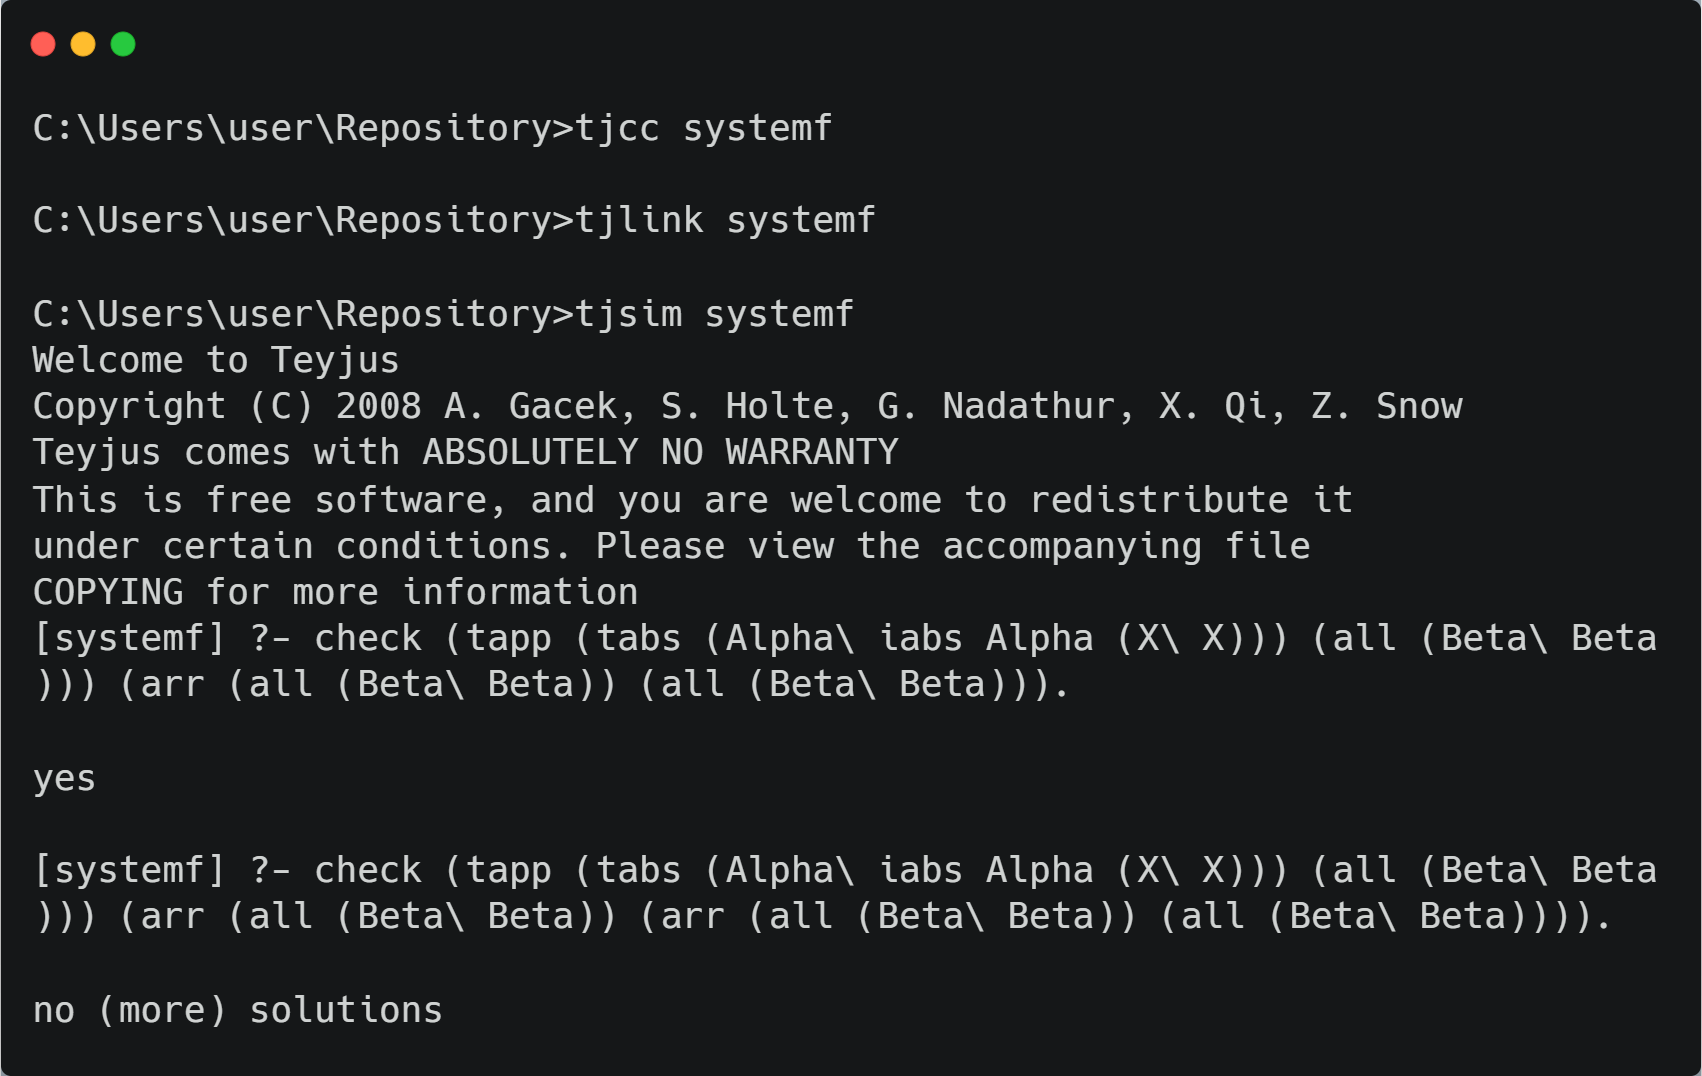
\includegraphics[width=0.9\linewidth]{fin.png}
            \end{center}
        \end{figure}
        \begin{itemize}
            \item 두 번째로 $\vdash \left( \Lambda \alpha . \lambda x^{\alpha} . x \right) \left( \forall \beta . \beta \right) : \left( \forall \beta . \beta \right) \to \left( \forall \beta . \beta \right) \to \left( \forall \beta . \beta \right)$인지 질의해보겠습니다.
            \item Teyjus V2는 ``no (more) solution''이라고 응답하는군요.
        \end{itemize}
    \end{frame}
    
    \begin{frame}
        \frametitle{이제 실행해봅시다.}
        \begin{figure}[h]
            \begin{center}
                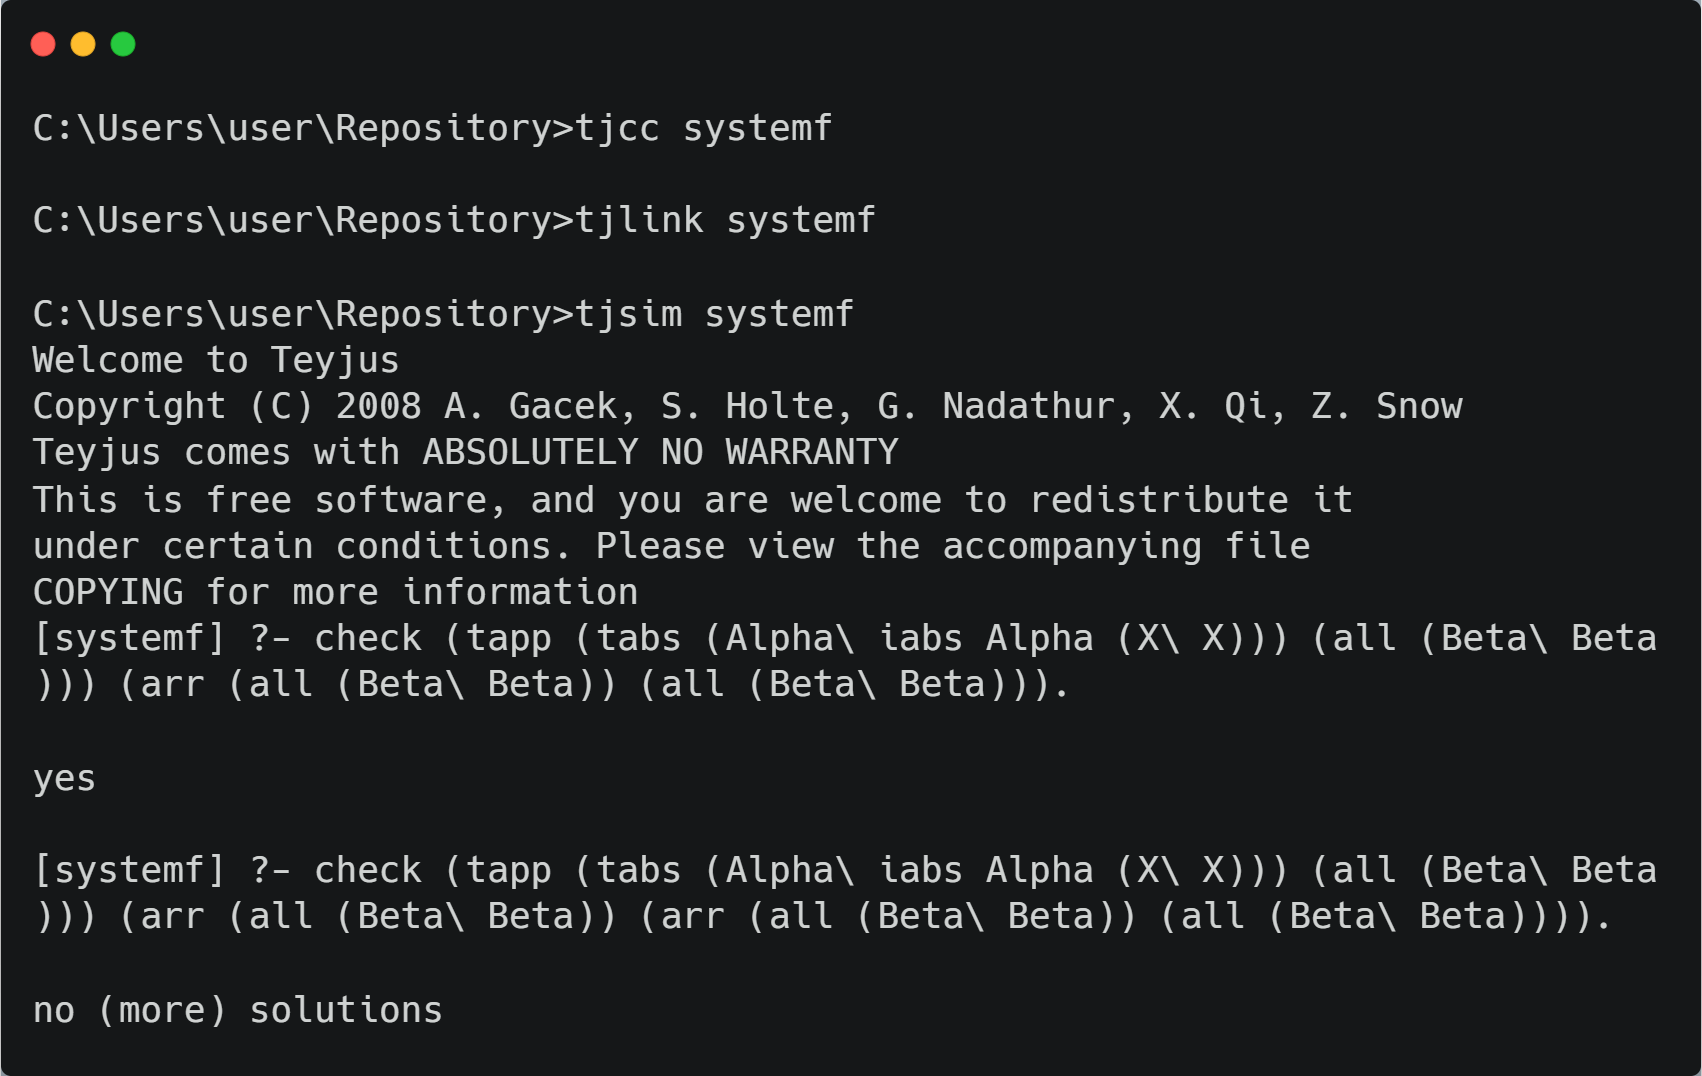
\includegraphics[width=0.9\linewidth]{fin.png}
            \end{center}
        \end{figure}
        \begin{itemize}
            \item 두 가지 질의에 대하여 모두 예상한 대로 응답함을 확인했습니다.
            \item 지금까지 경청해주셔서 감사합니다!
        \end{itemize}
    \end{frame}
\end{document}
